% TEMPLATE for Usenix papers, specifically to meet requirements of
%  USENIX '05
% originally a template for producing IEEE-format articles using LaTeX.
%   written by Matthew Ward, CS Department, Worcester Polytechnic Institute.
% adapted by David Beazley for his excellent SWIG paper in Proceedings,
%   Tcl 96
% turned into a smartass generic template by De Clarke, with thanks to
%   both the above pioneers
% use at your own risk.  Complaints to /dev/null.
% make it two column with no page numbering, default is 10 point

% Munged by Fred Douglis <douglis@research.att.com> 10/97 to separate
% the .sty file from the LaTeX source template, so that people can
% more easily include the .sty file into an existing document.  Also
% changed to more closely follow the style guidelines as represented
% by the Word sample file. 

% Note that since 2010, USENIX does not require endnotes. If you want
% foot of page notes, don't include the endnotes package in the 
% usepackage command, below.

% This version uses the latex2e styles, not the very ancient 2.09 stuff.

\documentclass[letterpaper,twocolumn,11pt]{article}
\usepackage{usenix,epsfig,endnotes,url,graphicx,multicol}
\graphicspath{{figures/}}
\begin{document}

%don't want date printed
\date{}

%make title bold and 14 pt font (Latex default is non-bold, 16 pt)
\title{\Large \bf CS217B Project Report: NDN Open mHealth Pilot Applications}

%for single author (just remove % characters)
\author{
{\rm Zhehao Wang, 404380075}\\
zhehao@cs.ucla.edu
} % end author

\maketitle

% Use the following at camera-ready time to suppress page numbers.
% Comment it out when you first submit the paper for review.
\thispagestyle{empty}

\section{Introduction}

Mobile health has emerged as both an important commercial market and a key area of Health IT, a national priority \cite{JeffBTechReport}.
%Within the many applications of mobile technology to health, Open mHealth focuses on leveraging the public’s everyday mobile devices to extend evidence based interventions beyond the reach of traditional care and thereby improve disease management and prevention. 
The Open mHealth team envisions that the Internet will interconnect data capture, secure storage, modeling and analytics, and user interface components to create a modular, layered framework. In \cite{SimEstrin2010}, the Open mHealth architecture uses a data-centric hourglass model, with the ``thin waist'' representing the storage unit and standardized data exchange. The focus on data exchange as the backbone of the application ecosystem makes Open mHealth an excellent network environment to both drive and evaluate NDN \cite{NPTechReport}.

% Open mHealth is one of the two network environments that the NDN project team proposed for ``Next Phase'' research from 2014-2016. 

The design work is mostly done in 2015, and this quarter's work focuses on the implementation side, with the goals being to create a demonstrable system which incorporates name based access control for data confidentiality, DPU data encapsulation, and producer mobility support in all the involved components. The first goal two goals are achieved and demonstrated in sample components, and the work on the last goal is still ongoing.

The goal of this project is to provide a working set of application components for the NDN Open mHealth (NDN omh) system, and in doing so, identify requirements for the architecture, and put new library features to test. For example, all components in the system would be customers for schematized trust \cite{SchematizedTrust}, name based access control (NAC)\cite{NACTR}, link objects, etc.

% what you have done and in particular what you have learned

\section{Progress this quarter}

The major components and dataflow of NDN omh are shown in Figure \ref{fig:dataflow}. Data storage units (DSU) serve as passive repositories for user's health data, and other user information such as their certificates and associated link objects. Data processing units (DPU) are user-authorized processing units, which consume users' raw data and produce processed data. The current system uses NFN for DPU \cite{NFN}. Data visualization units (DVU) are consumers in the system, and provide visualization to user's health data.

\begin{figure}[h]
\centering
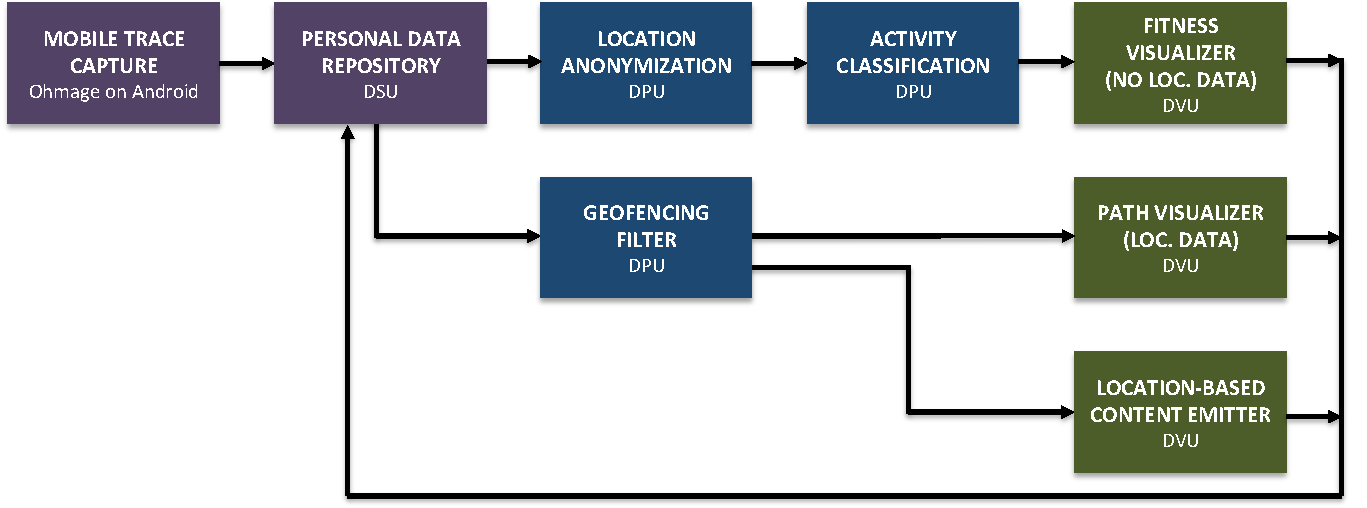
\includegraphics[width=0.45\textwidth]{ConceptualBlock.pdf}
\caption{NDN omh components and dataflow \cite{JeffBTechReport}}
\label{fig:dataflow}
\end{figure}

Since the last quarter progress has been made towards the mobile data producer, mobile identity manager and trust configuration, and the DSU. Initial incorporation of NFN is done during the 2016 Hackathon, though the resulting work didn't incorporate access control at that point. 

This quarter's implementation includes the following, and the following subsections introduce the implementation details worth mentioning.

\begin{itemize}
\item A sample producer in Python which puts encrypted user health data into DSU
\item A sample authorization manager in Python which receives access requests to user's data, decides if access should be granted, and serves as a group manager for NAC. The authorization manager also publishes the group's E-key and distributes each member's encrypted D-key.
\item A sample DPU in Python which requests access for user data, and consumes raw data to produce processed data on command interest.
\item A browser DVU in JavaScript which requests access for user data, decrypts user data and visualize, initiates DPU processing, and visualize all the data names in the network.
\end{itemize}

\subsection{Sample producer}

This producer is a simplified version of NDNFit Android application. It produces random time-location data for a pre-configured user, puts the produced data into its own memory content cache, and initiates DSU insertion, which is an NDN repository running repo-ng. The producer can be configured to produce encrypted data, in which case it'll issue interest for the E-keys of groups whose name is a prefix of the produced data name, verify the received E-keys, and publish the C-keys encrypted with each of the E-keys to the DSU.

The producer is built with PyNDN, whose NAC support is a direct port from Yingdi's version in C++. During the implementation of producer (in Hackathon) we identified an issue with both versions of NAC library, which wrongfully rounds the produced data's timestamp and causes the producer's finest time granularity to be every hour. This seems to be a simple implementation oversight, and was quickly fixed during the Hackathon. A separate issue is the exclusion mechanism with which the library fetches E-keys: whether the exact hour point is included or excluded. For our demonstration the behavior is changed to inclusive rather than the exclusive version in the library, so that a E-key for an hour period can cover the data produced at the exact starting hour. This issue's still pending in the library implementation.

The incorporation of NAC into the Android producer is still being tested.

\subsection{Sample authorization manager}

This authorization manager derives from the group manager in NAC, which provides interfaces for adding a member certificate to the group, and generating all the group keys (one group E-key and all D-keys for all members of the group). Access request and member certificate fetching are considered application-specific logic, and are out of the scope of the NAC library. This group manager receives membership request interests, which contain the name of the requesting identity's certificate. It then asks for the cetificate and grants access to anyone verifiable from a pre-installed anchor.

During the implementation of the group manager, we found a potential issue with the library's implementation of \textit{groupManager.getGroupKey}, the interface which returns the E-key of the group and all current member's D-keys. The current implementation regenerates all key pairs upon each call, which in our case would invalidate the C-key encrypted with a previous E-key, and the producer has to be aware of the new E-key each time this function is called (which needs to happen every time a new member's added, in order to publish that member's encrypted D-key). For our demonstration, the behavior of this function is changed to only generate E-key once, and upon each call only generate D-keys for members whose D-keys don't previously exist. This potential issue's still pending in the library implementation.

We expect the actual authorization manager to also be an Android application running on the same device as the producer application, and the authorization manager would contain multiple group managers and an access request interface, which upon receiving requests, would allow user to choose who to grant access to (instead of relying on a pre-installed trust schema), in which group, and for how long.

\subsection{Sample DPU}

Our sample DPU operates under its organization namespace: it receives command interests in its organization namespace, and wants to produce data available in the user namespace. To achieve this the DPU produces data under the organization namespace, so that the command interest is satisfiable, and in the data is another data packet under the user namespace, so that the receiving end, or the DPU itself can put it in DSU and make it available under the user namespace; both outer and inner data are signed by DPU's key. For our demo, calling the function with the following outer name
\begin{verbatim}
/ndn/edu/basel/dpu/bounding_box
(<userid>, <timestamp>, <inner_data_name>)
\end{verbatim} 
will generate the inner name that looks like the following
\begin{verbatim}
/org/openmhealth/<userid>/data/fitness
/physical/processed_result
/bounding_box/<timestamp>
\end{verbatim}
in the parameters \verb|<userid>| and \verb|<timestamp>| are mandatory, and \verb|<inner_data_name>| is optional if the caller wants to further customize the generated inner data name.

In addition to doing encapsulation, the DPU also serves as both a NAC consumer and producer. As a consumer it first requests access, then fetch the catalog, and using names in the catalog to ask for data and the correct credentials to decrypt the C-key. As a producer it respects the data owner's group setup by requesting the same E-keys thus making sure the same groups have access to the data.

The implementation of DPU shares the same potential library issues with the sample producer, with the same revisions on the library as described previously, we were able to implement a DPU that provides a simple bounding box function.

Ideally we want to use an NFN component as the DPU, but the incorporation of NAC into NFN is still being tested.

\subsection{DVU}

The DVU runs in browser and provides the options of requesting user data access, fetching a user's raw or processed data, initiating DPU processing with a given name, and show all data names in the network (organized as a tree). The implementation uses ndn-js's port of NAC, which did not require any direct change since the consumer implementation in NAC is working as expected.

\subsection{Demo setup and names involved}

This section describes the process and names involved in the initial demo of the system \footnote{Which can be found at: https://www.youtube.com/watch?v=3l2w30rZqdk; and the corresponding implementation is https://github.com/zhehaowang/sample-omh-dpu}. Figure \ref{fig:nac} introduces the sequence of events in the demo, featuring the access granting and raw data consumption part. 

\begin{figure}[h]
\centering
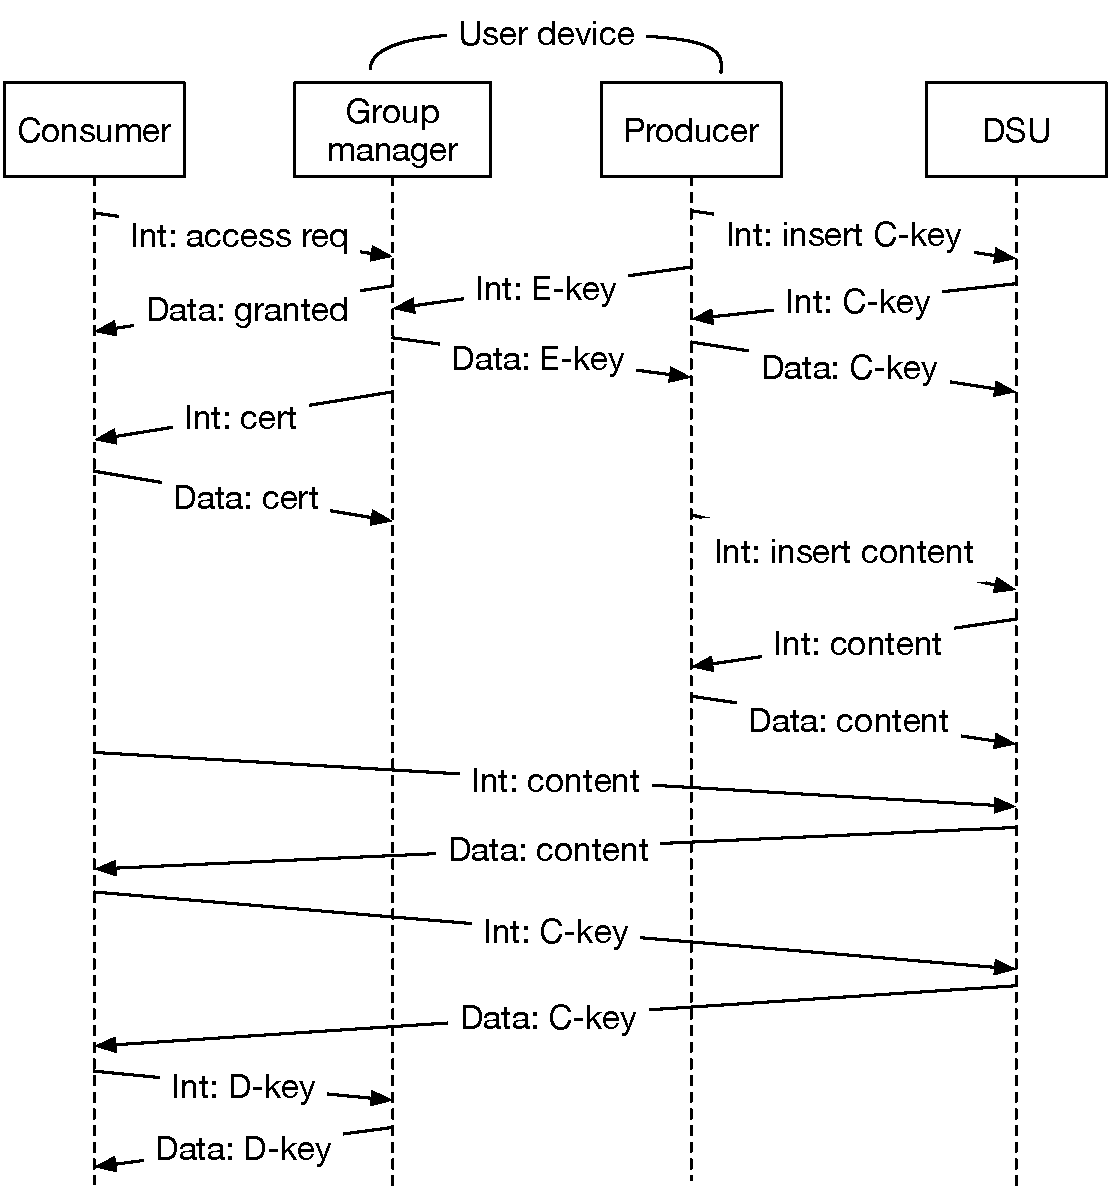
\includegraphics[width=0.45\textwidth]{nac-steps.pdf}
\caption{NAC demo workflow}
\label{fig:nac}
\end{figure}

And the names involved include: 
\begin{itemize}
\item User namespace (group name): 
\begin{verbatim}
/org/omh/zhehao
\end{verbatim} 

\item Encrypted content name:
\begin{verbatim}
/org/omh/zhehao/SAMPLE/fitness/physical
/time_location/20160320T080058
/FOR
/org/omh/zhehao/SAMPLE/fitness/physical
/time_location/C-KEY/20160320T080000
\end{verbatim} 

\item Catalog name:
\begin{verbatim}
/org/omh/zhehao/data/fitness/physical
/time_location/catalog/20160320T080000
/%FD%01
\end{verbatim} 

\item DVU identity name: 
\begin{verbatim}
/org/omh/dvu-browser/
\end{verbatim} 

\item DVU access request interest:
\begin{verbatim}
/org/omh/zhehao/read_access_request
/org/omh/dvu-browser/KEY/ksk-1464919278
/ID-CERT/%FD%00%00%01U%13%FEC%BA/
%FD%00%00%01U%14t%E7%F9
\end{verbatim} 

\item Encrypted C-key:
\begin{verbatim}
/org/omh/zhehao/SAMPLE/fitness/physical
/time_location/C-KEY/20160320T080000
/FOR
/org/omh/zhehao/READ/fitness/E-KEY
/20160320T080000/20160320T100000
\end{verbatim} 

\item Group E-key name:
\begin{verbatim}
/org/omh/zhehao/READ/fitness/E-KEY
/20160320T080000/20160320T100000
\end{verbatim} 

\item Consumer D-key name:
\begin{verbatim}
/org/omh/zhehao/READ/fitness/D-KEY
/20160320T080000/20160320T100000
/FOR
/org/openmhealth/dvu-browser
/ksk-1464919278
\end{verbatim} 

\item DPU identity name: 
\begin{verbatim}
/ndn/edu/basel/dpu/
\end{verbatim} 

\item And DPU function call name and produced data names are given in the previous section.

\end{itemize}

\section{Conclusion}

What we achieved can be summarized as providing sample implementations for all the involved components, featuring name based access control and DPU data encapsulation; the details are introduced in previous section. This section discusses what we learnt and the immediate future work for the project this quarter.

\subsection{What we learnt}

What we've learnt can be summarized as the following bullets:

\begin{itemize}
\item Implementation experience: this project involves a considerable amount of implementation in multiple languages (mostly done in Python and JavaScript) and platforms (components are running on OSX, Ubuntu, Android and in browser), and the resulting implementation and integrationt testing experience is valuable. (The process of looking inside the library to debug is helpful, too, in understanding how exactly everything works)
\item NAC library usability: this application's also the first one that fully features the NAC library, whose debugging, for now, requires pretty detailed review of the code. We did identify a few potential issues, and hopefully could help improve the usability of NAC library, and provide a working example for other applications wishing to feature data confidentiality and access control.
\item Writing experience: earlier this quarter we did a short paper submission for ICN, which could serve as an initial documentation of the system design. Though the writing quality as a paper ends up being subpar, the process of finding selling points in the project and organizing the ideas to make them presentable is still helpful.
\item The process of designing, building a system, then identifying the problems and making improvements: this is something we are hoping to learn from building the NDN Open mHealth system, though we can't state that we've learnt a lot in this aspect, as the work this quarter can still be categorized as the initial stage of building the prototype. We are hoping to learn more from seeing the system in action, and evaluate/improve in the next iteration.
\end{itemize}

And as a side note, we did not run into many problems as other groups did when testing on the testbed, or installing dependencies, most likely because of the familiarity with existing tools, libraries and how they work.

\section{Future work}

Implementation and deployment wise, the immediate future work includes the following.

\begin{itemize}

\item Incorporating with real components: as discussed in the previous section, most of the components serve as sample implementations rather than real components to be demonstrated with the system. Some effort should go into actually building the components as we imagined (for example, the authorization manager in Android; and incorporating schematized trust as in the design document).

\item System deployment, evaluation and better visualization. With more initial implementations in place, we can move on with actual deployment on testbed, and decide how to best evaluate and demonstrate the system. The current idea's to visualize the interest and data exchange between different components, however, more thought needs to go into designing the demo so that it's clear and helpful, or better yet, to be able to evaluate with the IP implementation from certain aspects.

\end{itemize}

{\footnotesize \bibliographystyle{acm}
\bibliography{bibliography}}

\end{document}







